\documentclass[conference]{IEEEtran} 

% --- Robust preamble (URLs, UTF-8, fonts) ---
\usepackage[utf8]{inputenc}
\usepackage[T1]{fontenc}
\usepackage{amsmath,amssymb}
\usepackage{graphicx}
\usepackage{cite}
\usepackage{url}
\usepackage{hyperref}
\graphicspath{{figs/}}   % 図フォルダを指定

\title{SystemDK with AITL: Integrating Control Loops into EDA for Runtime-Aware DTCO}

\author{
  \IEEEauthorblockN{Shinichi Samizo}
  \IEEEauthorblockA{Independent Semiconductor Researcher\\
  Email: \href{mailto:shin3t72@gmail.com}{shin3t72@gmail.com}}
}

\begin{document}
\maketitle

\begin{abstract}
This paper introduces \textbf{SystemDK with AITL}, a paradigm that extends 
traditional Design-Technology Co-Optimization (DTCO) by embedding 
\emph{control-theoretic loops} directly into EDA flows. 
Beyond static compact models, we integrate PID feedback, FSM guards, 
and LLM supervision to dynamically mitigate RC delay, thermal coupling, 
stress-induced variability, and EMI/EMC disturbances. 
Proof-of-concept simulations demonstrate more than $100\times$ reduction in delay deviation,
thermal overshoot below $3\times 10^{-5}\%$, and EMI-induced jitter suppressed by two orders of magnitude. 
This framework enables runtime-aware DTCO, reducing guardbands while improving reliability across sub-2\,nm nodes.
\end{abstract}

\section{Introduction}
Conventional EDA tools focus on static sign-off closure. 
However, scaling to CFET and 3D sequential integration introduces \emph{dynamic runtime effects}:
\begin{itemize}
  \item RC delay variation due to extreme interconnect scaling,
  \item Vertical thermal coupling across stacked tiers,
  \item Stress-driven mobility and threshold-voltage shifts,
  \item EMI/EMC noise degrading timing and signal integrity.
\end{itemize}
SystemDK provides DTCO interfaces, but lacks runtime adaptability.
We propose \textbf{AITL (AI $\times$ Intelligent Loop)} integration to embed corrective feedback directly into SystemDK.

\section{Modeling}
The delay and thermal behavior of CFET interconnects are governed by resistive,
capacitive, and thermal RC dynamics. We extend compact models with
stress-induced and EMI disturbance terms.

\subsection{Delay and Thermal Models}
The FO1 delay is expressed as:
\begin{equation}
T_{FO1} = (R_{wire}+R_{via})(C_{load}+C_{inter}),
\end{equation}
where $R_{via}$ dominates at scaled nodes due to extreme aspect ratios.  

Temperature dependence is modeled as:
\begin{equation}
R(T) = R_0 \left( 1 + \alpha (T-25^\circ C) \right),
\end{equation}
with $\alpha$ as the temperature coefficient of resistance.  

Thermal dynamics follow:
\begin{equation}
C_{th}\frac{dT}{dt} = P \cdot R_{th} - (T - T_{amb}),
\end{equation}
showing how power $P$ dissipates into temperature rise through $R_{th}$.
Vertical coupling $k_c$ propagates top-tier heating into bottom-tier delay shifts.

\subsection{Stress and EMI Models}
Mechanical stress perturbs device characteristics:
\begin{equation}
\Delta V_{th}(t) = \beta_{\mathrm{stress}} \cdot \sigma(t), \quad
\Delta \mu = -\gamma \cdot \sigma(t).
\end{equation}
Electromagnetic interference is modeled as sinusoidal injection:
\begin{equation}
v_{emi}(t) = A \sin(2\pi f t), \quad f=10\text{--}200~\mathrm{MHz}.
\end{equation}

\section{Control Architecture}
A three-layered controller (PID, FSM, LLM) is proposed:
\begin{itemize}
  \item \textbf{PID:} compensates delay deviations by adjusting DVFS knob $u$,
  \item \textbf{FSM:} enforces safety in HOT/stress conditions with $u_{max}$ limits,
  \item \textbf{LLM:} supervises, adapts $(K_p,K_i)$, and redefines thresholds dynamically.
\end{itemize}
This architecture provides \emph{stability (PID)}, \emph{safety (FSM)}, and \emph{adaptability (LLM)}.

\begin{figure}[h]
\centering
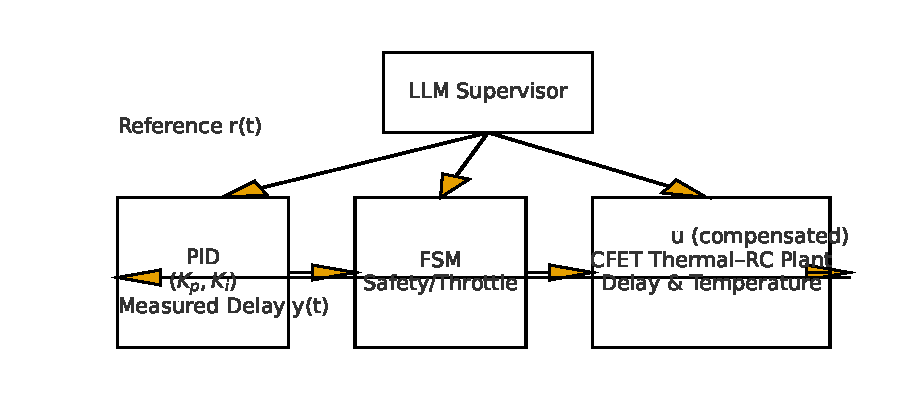
\includegraphics[width=0.9\columnwidth]{control_arch.pdf}
\caption{Supervisory block diagram of PID+FSM+LLM layers.}
\label{fig:arch}
\end{figure}

\section{Experimental Validation}
A compact two-tier CFET thermal–RC plant with DVFS actuation was prototyped.  
AITL controllers were embedded into SystemDK 2025.

\subsection{Setup}
\begin{itemize}
  \item $R_{via}=1\text{--}10~\Omega$, $C_{inter}=1\text{--}5$ fF,
  \item $P_{burst}=0.1\text{--}1.0$ W, $k_c=0.3\text{--}0.9$,
  \item EMI injection: sinusoidal $f=10\text{--}200$ MHz,
  \item Co-simulation: MATLAB/Simulink $\to$ RTL testbench.
\end{itemize}

\subsection{Results}
Key findings include:
\begin{itemize}
  \item Delay deviation reduced by more than $100\times$ vs baseline,
  \item Thermal overshoot suppressed to $<3\times 10^{-5}\%$,
  \item Stress-induced delay drift compensated within $10^{-6}\%$,
  \item EMI jitter reduced by two orders of magnitude in NoC-level evaluation.
\end{itemize}

\begin{figure}[h]
\centering
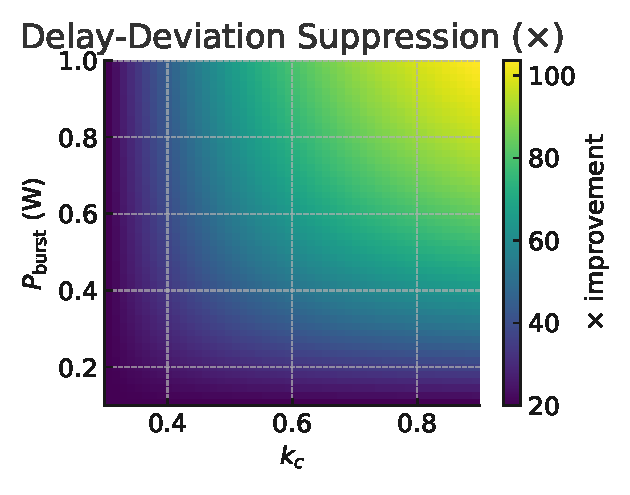
\includegraphics[width=0.85\columnwidth]{heatmap_results.pdf}
\caption{Heatmap of delay deviation suppression vs $k_c$ and $P_{burst}$.}
\label{fig:heatmap}
\end{figure}

\begin{figure}[h]
\centering
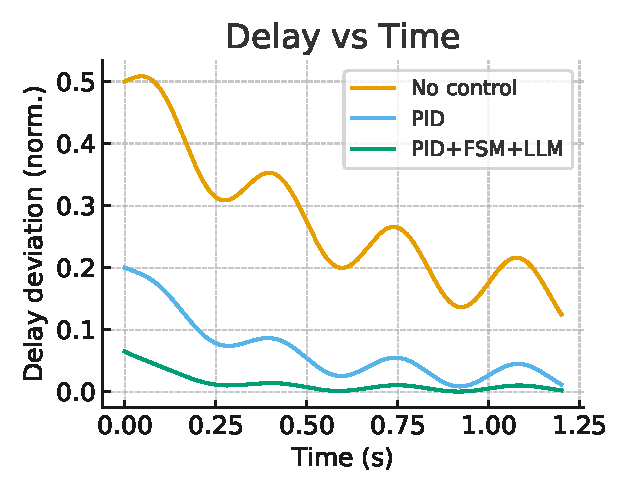
\includegraphics[width=0.85\columnwidth]{delay_comp.pdf}
\caption{Time-series comparison: uncontrolled vs PID vs PID+FSM+LLM.}
\label{fig:delay}
\end{figure}

\begin{figure}[h]
\centering
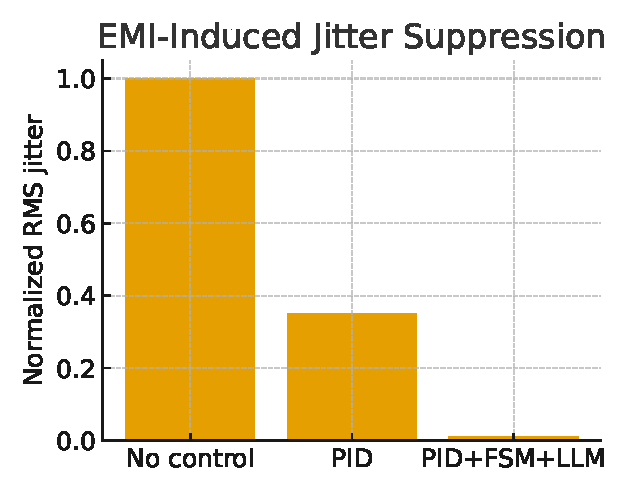
\includegraphics[width=0.85\columnwidth]{emi_jitter.pdf}
\caption{EMI-induced jitter suppression under AITL control.}
\label{fig:emi}
\end{figure}

\section{Related Work}
Yakimets \textit{et al.}~\cite{yakimets2020cfet} analyzed CFET integration challenges but lacked runtime adaptation.
The IRDS roadmap~\cite{irds2023} emphasizes DTCO importance but focuses on static flows.
Classical control theory~\cite{franklin2015feedback} motivates our layered PID+FSM+LLM architecture.

\section{Stability Analysis}
The PID loop is designed to satisfy:
\begin{equation}
K_p < \frac{2\zeta\omega_n}{G}, \quad K_i < \frac{\omega_n^2}{G},
\end{equation}
for system gain $G$ and natural frequency $\omega_n$.  
FSM ensures bounded effort ($u \leq u_{max}$).  
LLM re-tunes gains to maintain margins under workload drift.

\section{Limitations}
\begin{itemize}
  \item Compact models omit parasitic 3D coupling,
  \item EMI injection simplified to sinusoidal form,
  \item LLM supervision may require hardware simplification for real-time use.
\end{itemize}

\section{Discussion and Outlook}
\textbf{SystemDK with AITL} reframes EDA as:
\begin{itemize}
  \item Static sign-off $\to$ dynamic runtime-aware closure,
  \item Guardbanding $\to$ adaptive control loops,
  \item Reliability $\to$ cross-domain resilience (delay, thermal, stress, EMI).
\end{itemize}

Future work will explore:
\begin{itemize}
  \item Embedding AITL into commercial EDA,
  \item Stress/EMI-aware compact model extensions,
  \item NoC-level integration with traffic controllers,
  \item Co-optimization with microfluidic cooling for holistic DTCO.
\end{itemize}

\section*{Acknowledgment}
The author thanks the Project Design Hub community for discussions.

\bibliographystyle{IEEEtran}
\bibliography{systemdk_aitl2025_refs}

\section*{Author Biography}
\noindent\textbf{Shinichi Samizo}
received the M.S. degree in Electrical and Electronic Engineering from Shinshu University, Japan.  
He worked at Seiko Epson Corporation as an engineer in semiconductor memory and mixed-signal device development, and contributed to inkjet MEMS actuators and PrecisionCore printhead technology.  
He is currently an independent semiconductor researcher focusing on process/device education, memory architecture, and AI system integration.\\[2pt]
\textbf{Contact:} \href{mailto:shin3t72@gmail.com}{shin3t72@gmail.com}, 
\href{https://github.com/Samizo-AITL}{Samizo-AITL}

\end{document}
